% More info on this class can be found on: http://www.ctan.org/pkg/paper.
\documentclass[12pt,a4paper,oneside]{paper} % Accepts option `twocolumn`.
%\usepackage{fullpage} % If needed.
\usepackage{lmodern} % Fonts. Needed somehow, otherwise things break.
\usepackage[english]{babel} % English language/hyphenation.
\usepackage[T1]{fontenc} % Use 8-bit output encoding.
\usepackage[utf8]{inputenc} % Can use UTF-8 in the source files.
\usepackage[babel]{microtype} % Improves appearance of text.
\usepackage{url}
\usepackage{csquotes}
\usepackage{float}
\usepackage[]{minted}
\usepackage{amsmath,amsthm, amssymb}
% Reference sheet: http://merkel.zoneo.net/Latex/natbib.php
% \usepackage{natbib} % Better references
% \bibliographystyle{abbrvnat}
% If possible, it is preferable to directly include PDF images.
\usepackage{graphicx}
\graphicspath{{fig/}}
\usepackage{hyperref}
\hypersetup{
  colorlinks=false,
  pdfauthor={Gaurav Gupta},
  pdftitle={Assignment 1: Forumulation of Optimization Problems}
}

%creates a new question command
\newcommand{\question}{%
    \stepcounter{section}% Increment the section counter
    \section*{Question \thesection}% Print "Question" followed by the updated section number
    \addcontentsline{toc}{section}{Question \thesection}% Optionally add to the table of contents
}

\newcommand{\variables}{%
    {\subsection{Decision Variables}} % Smaller font for subsection title
    \addcontentsline{toc}{subsection}{Decision Variables}
}

\newcommand{\constraints}{%
    {\subsection{Constraints}} % Smaller font for subsection title
    \addcontentsline{toc}{subsection}{Constraints}
}

\newcommand{\of}{%
    {\subsection{Objective Function}} % Smaller font for subsection title
    \addcontentsline{toc}{subsection}{Objective Function}
}

\newcommand{\sol}{%
    {\subsection{Solution}} % Smaller font for subsection title
    \addcontentsline{toc}{subsection}{Solution}
}

% Removes double spacing after end of sentence.
% See: http://practicaltypography.com/one-space-between-sentences.html.
\frenchspacing


\title{Assignment 1: Forumulation of Optimization Problems}
\subtitle{AE413: Optimization techniques in engineering}
\author{Gaurav Gupta, SC21B026}

% Don't know how this is used. Removing it messes the header.
\shortauthor{Gaurav}
\shorttitle{Assignment 1}

\begin{document}
\maketitle

% \abstract{}
\question{}
\label{sec:intro}
\variables{}
The launch angle of elevation ($\theta$) is the decision variable here with a range of $[0^{\circ}, 80^{\circ}]$. The parameters $h$ and $V$ are given as $50$m and $90$ m/s.

\begin{figure}[H]
  \centering
  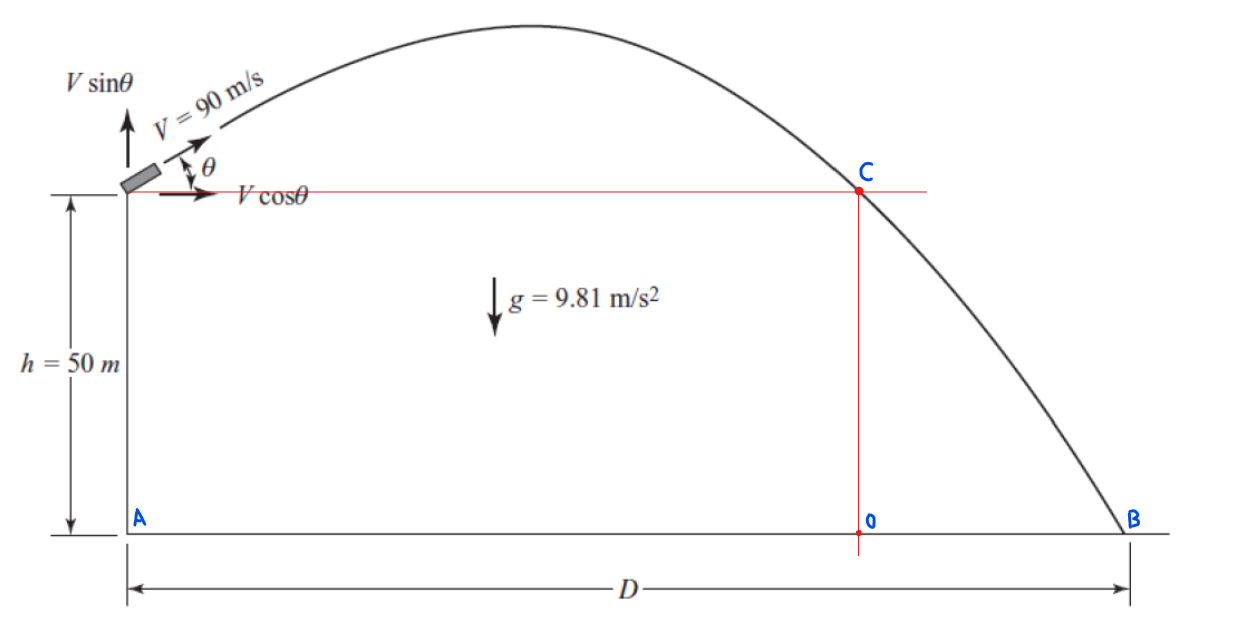
\includegraphics[width=\textwidth]{q1.png}
  \caption{Trajectory for the projectile}
  \label{fig:example}
\end{figure}

\of{}
The range of the projecticle is to be maximized in the question. The range $(D)$ is divided into two segments $AO$ and $OB$ as shown in the Figure \ref{fig:example}.

$$
  AO = \text{Range} = \frac{V^2 sin(2\theta)}{g}
$$

At point C, $u = Vsin\theta$, $a=g$ and $s=h$, then using the equations of motion.


\begin{align*}
  s  & = ut + \frac{1}{2}at^2                                                                    \\
  h  & = Vtsin\theta + \frac{1}{2}gt^2                                                           \\
  t  & = \frac{-2Vsin\theta + \sqrt{4V^2sin^2\theta + 2hg}}{2g}                                  \\
  OB & = vcos\theta \left(\frac{-Vsin\theta}{g} + \sqrt{\frac{V^2sin^2\theta + 2hg}{g^2}}\right)
\end{align*}


Therefore,
$$
  D = AO + OB =  \frac{V^2 sin(2\theta)}{2g} + Vcos\theta \sqrt{\left(\frac{Vsin\theta}{g}\right)^2 + \frac{2h}{g}}
$$

\sol{}

\begin{minted}[linenos, breaklines, breakanywhere]{matlab}
%Question1
clc; clear;
lb1=0; ub1=80*pi/180; %Constraints on theta
u=90; h=50; %Initial conditions of objective function
options=optimoptions("fmincon","Display","iter","TolFun",1e-8,"TolX",1e-8,"MaxIter",10000);
fun1=@(x)obj1(x,u,h);
theta0=45*pi/180;
[theta,fval]=fmincon(fun1,theta0,[],[],[],[],lb1,ub1,[],options);

theta=theta*180/pi; D=-fval;


function F=obj1(x,u,h)
g=9.81;
F=-u*cos(x)*((u/g)*sin(x)+sqrt(2*(h/g)+((u/g)*(u/g)*sin(x)*sin(x))));
end
\end{minted}
\vspace{0.5cm}
\noindent The maximum value for $D$ is $874.259$ m for the value of $\theta=43.363^{\circ}$.

\question
\variables
\begin{itemize}
  \item $\mathbf{i}$ : Manufacturing facilities, where $i \in \{1,2,..m\}$.
  \item $\mathbf{j}$ : Retailer, where $j \in \{1,2,..n\}$.
  \item $\mathbf{k}$ : Locations for setting manufacturing facilities, where $k \in \{1,2,..p\}$.
  \item $\mathbf{Q_{ij}}$ : Quantity supplied by $i^{th}$ factory to $j^{th}$ retailer.
  \item $\mathbf{C_{kj}}$ : Cost of tranportation of goods from location $k$ to retailer $j$  .
  \item $\mathbf{A_{ki}}$ : Assignment of location $k$ to factory $i$. It is a binary variable with possible values as $0$ and $1$.
        \[ A_{ki} = \begin{cases}
            1 & \mbox{ if location $k$ is assigned to factory $i$} \\
            0 & \mbox{ otherwise}
          \end{cases}
        \]
\end{itemize}
\constraints
\begin{enumerate}
  \item A location should be alloted to only one factory, then
        $$
          \sum_{i=1}^{m} A_{ki}\le 1\;\;\forall\; k \in \{1, 2, 3, 4, ..., p\}
        $$
  \item Each factory should be accomodated at one location only, then
        $$
          \sum_{k=1}^{p} A_{ki}=1\;\;\forall\; i \in \{1, 2, 3, 4, ..., m\}
        $$
\end{enumerate}
\of
The cost of tranportation from factory $i$ to retailer $j$, if location $k$ is selected is $A_{ki}Q_{ij}C_{kj}$.
$$
  \text{Minimize}\;\sum_{k=1}^{p} \sum_{j=1}^{n} \sum_{i=1}^{m} A_{ki}Q_{ij}C_{kj}
$$
\newpage
\sol
\begin{minted}[linenos, breaklines]{python}
i = 3
j = 2
k = 5
Qij = [10, 7, 15, 20, 15, 8]
Ckj = [100, 200, 250, 150, 400, 450, 300, 150, 250, 300]
Aki = np.zeros((1, k * i))

bounds = Bounds(0, 1)  # 0 <= x_i <= 1
integrality = np.ones(15)  # 15 integer variables

# Coefficient Matrix
c = (np.reshape(Ckj, (k, j)) @ np.reshape(Qij, (j, i)))
c = c.flatten()

# Constraints
# A1: Ensuring each k row has a sum of 1
A1 = np.zeros((k, i * k))
for n in range(k):
    A1[n, n * i:(n + 1) * i] = 1

B1_u = np.ones(k)
B1_l = -np.inf * np.ones(k)

# A2: Sum constraints for i elements across different k
A2 = np.zeros((i, i * k))
for n in range(i):
    A2[n, n::i] = 1

B2_u = np.ones(i)
B2_l = np.copy(B2_u)

# Combining constraints
A = np.vstack([A1, A2])
b_u = np.hstack([B1_u, B2_u])
b_l = np.hstack([B1_l, B2_l])

cons = LinearConstraint(A, b_l, b_u)
res = milp(c=c, integrality=integrality, bounds=bounds, constraints=cons)
\end{minted}
\vspace{0.5cm}
\noindent Minimum cost of tranportation is Rs. 12950 for the above problem. $A_{ki}$ matrix for the above problem is

$$ A_{ki} = 
\begin{bmatrix}
  0 & 0 & 1\\
  1 & 0 & 0\\
  0 & 0 & 0\\
  0 & 1 & 0\\
  0 & 0 & 0\\
\end{bmatrix}
$$

\question{}
\variables
\begin{itemize}
  \item $\mathbf{i}$ : Grower, where $i \in \{1,2,3\}$.
  \item $\mathbf{j}$ : Plant to be supplied, where $j \in \{1,2\}$.
  \item $\mathbf{Q_{ij}}$ : Quantity of fruits supplied by $i^{th}$ grower to $j^{th}$ plant.
  \item $\mathbf{S_{ij}}$ : Shipping cost from $i^{th}$ grower to $j^{th}$ plant.
  \item $\mathbf{r_i}$ : Rate of fruits/tonne supplied by $i^{th}$ grower.
  \item $\mathbf{G_i}$ : Maximum quantity of fruits supplied by $i^{th}$ grower.
  \item $\mathbf{C_j}$ : Capacity of $j^{th}$ plant.
  \item $\mathbf{L_j}$ : Labour cost of $j^{th}$ plant.
\end{itemize}

\constraints
\begin{enumerate}
  \item Sum of fruits supplied to the plant should be less than or equal to their total capacity.
        $$
          \sum_{i=1}^{3} Q_{ij} \le C_{j}\;\; \forall\;j\in\{1,2\}
        $$
  \item Sum of fruits supplied by each grower should not exceed their maximum limit.
        $$
          \sum_{j=1}^{2} Q_{ij} \le G_{i}\;\; \forall\;i\in\{1,2,3\}
        $$
\end{enumerate}

\of
Cost of production for fruits supplied by $i^{th}$ grower to $j^{th}$ plant is $Q_{ij}(r_i + S_{ij} + L_j)$. Thus, the profit is $Q_{ij}(50000 - r_i - S_{ij} - L_j)$.

$$
  \text{Maximize}\;\; \sum_{j=1}^{2} \sum_{i=1}^{3} Q_{ij}(50000 - r_i - S_{ij} - L_j)
$$

\sol
\begin{minted}[linenos, breaklines]{python}
# Given data
ri = np.array([1100, 1000, 900])
Sij = np.array([[3000, 3500], [2000, 2500], [6000, 4000]])
Gi = np.array([200, 310, 420])
Cj = np.array([460, 560])
Lj = np.array([26000, 21000])

# Number of suppliers and plants
num_suppliers = 3
num_plants = 2

# Objective function coefficients (profit per unit)
selling_price = 50000
c = -(
    selling_price -  # Revenue
    np.repeat(ri, num_plants) -  # Supplier cost
    Sij.flatten() -  # Shipping cost
    np.tile(Lj, num_suppliers)  # Labor cost
)

# Inequality constraints (Ax <= b)
A_ub = []

# Plant capacity constraints: Sum of supplies to each plant <= Plant capacity
for j in range(num_plants):
    constraint = np.zeros(num_suppliers * num_plants)
    for i in range(num_suppliers):
        constraint[i * num_plants + j] = 1
    A_ub.append(constraint)

b_ub = Cj.tolist()  # Plant capacities

# Supplier capacity constraints: Sum of supplies from each supplier <= Supplier capacity
for i in range(num_suppliers):
    constraint = np.zeros(num_suppliers * num_plants)
    for j in range(num_plants):
        constraint[i * num_plants + j] = 1
    A_ub.append(constraint)

b_ub.extend(Gi.tolist())  # Supplier capacities

# Convert to numpy arrays
A_ub = np.array(A_ub)
b_ub = np.array(b_ub)

# Bounds for each variable (non-negative quantities)
bounds = [(0, None)] * (num_suppliers * num_plants)

# Initial guess (not used in linprog, but defining for clarity)
initial_guess = np.zeros(6)

# Perform linear programming optimization (linprog minimizes, so we negate c for maximization)
result = linprog(c, A_ub=A_ub, b_ub=b_ub, bounds=bounds, method='highs')

# Reshape the result to a 2D array
Q_opt = result.x.reshape(num_suppliers, num_plants)

# Print the results
max_profit = -result.fun  # Negate because we minimized the negative profit
\end{minted}

\vspace{0.5cm}
\noindent The maximum profit is Rs. 21242000.

\begin{table}[H]
  \centering
  \begin{tabular}{||c|c|c||}
    \hline
                        & \textbf{Plant A} & \textbf{Plant B} \\
    \hline
    \textbf{Supplier 1} & 200              & 0                \\
    \hline
    \textbf{Supplier 2} & 170              & 140              \\
    \hline
    \textbf{Supplier 3} & 0                & 420              \\
    \hline
  \end{tabular}
\end{table}

\question
\variables
\begin{itemize}
  \item $\mathbf{i}$ : Type of acid, where $i \in \{1,2\}$
  \item $\mathbf{j}$ : Type of operation, where $j \in \{1,2\}$
  \item $\mathbf{Q_i}$ : Quantity of $i^{th}$ acid.
  \item $\mathbf{M_j}$ : Maximum time available on $j^{th}$ operation.
  \item $\mathbf{P_i}$ : Profits from selling $i^{th}$ acid.
  \item $\mathbf{Q_3}$ : Quantity of by-product C sold.
  \item $\mathbf{Q_4}$ : Quantity of by-product C destroyed.
  \item $\mathbf{P_3}$ : Profit from selling C.
  \item $\mathbf{P_4}$ : Destruction cost of C.
  \item $\mathbf{T_{ij}}$ : Time required to manufacture $i^{th}$ acid using $j^{th}$ operation.
\end{itemize}
\constraints
\begin{enumerate}
  \item Operation Time Constraint
        $$
          \sum_{i=1}^{2} Q_i T_{ij} \le M_j \; \forall\; j \in \{1,2\}
        $$
  \item By-product constraint
        $$
          Q_2 = n(Q_3 + Q_4)
        $$
  \item Maximum forecasted sale of K units of by-product c
        $$
          0 \le Q_3 \le K
        $$
\end{enumerate}
\of
$$
  \text{Maximize}\;\; \sum_{i=1}^{2} Q_i P_i + P_3 Q_3 - P_4 Q_4
$$

\sol
\begin{minted}[linenos, breaklines]{python}
i = 2
j = 2
Mj = [20, 18]
Tij = [3, 4, 3, 2]
Pi = [200, 300]     # Profit coefficients for i
P3 = 150            # Profit coefficient for P3
P4 = 75             # Profit coefficient for P4
n = 5               # By-product multiplier

# Coefficient matrix for objective function
c = -np.array(Pi + [P3, -P4])

# Boundaries for the decision variables (x1, x2, x3, x4 >= 0)
bounds = [(0, None)] * 4

# Inequality constraint (time constraint): Tij @ x <= Mj
Au = np.array([[Tij[0], Tij[2], 0, 0],
               [Tij[1], Tij[3], 0, 0]])

Bu = np.array(Mj)

# Equality constraint (by-product constraint): x2 - n * (x3 + x4) = 0
Aeq = np.array([[0, 1, -n, -n]])
Beq = np.array([0])

# Solving the optimization problem
res = linprog(c, A_ub=Au, b_ub=Bu, A_eq=Aeq, b_eq=Beq, bounds=bounds)
\end{minted}

\noindent The maximum profit for the above problem is Rs. 2125 with the produced value of acid and the by-products as follows,

\begin{table}[H]
  \centering
  \begin{tabular}{||c|c||}
    \hline
    Acid A & 0\\\hline
    Acid B & 6.667\\
    \hline
    By-product C sold & 1\\
    \hline
    By-product D destroyed & 0.333\\
    \hline
  \end{tabular}
\end{table}

\question
\variables
\begin{itemize}
  \item $\mathbf{i}$ : Bin, where $i \in \{1,2,3,..,m\}$
  \item $\mathbf{j}$ : Items, where $j \in \{1,2,3,..,n\}$
  \item $\mathbf{V_j}$ : Volume of $j^{th}$ item.
  \item $\mathbf{W_j}$ : Weight of $j^{th}$ item.
  \item $\mathbf{A_{ji}}$ : Assignment of $j^{th}$ item to $i^{th}$ bin. It is a binary variable with possible values as $0$ and $1$.
        \[ A_{ki} = \begin{cases}
            1 & \mbox{ if item $j$ is assigned to bin $i$} \\
            0 & \mbox{ otherwise}
          \end{cases}
        \]
\end{itemize}

\constraints
\begin{enumerate}
  \item Volume Constraint
        $$
          \sum_{j=1}^{n} A_{ji} V_j \le V \; \forall\; i \in \{1,2,3,..,m\}
        $$
  \item Weight Constraint
        $$
          \sum_{j=1}^{n} A_{ji} W_j \le W \; \forall\; i \in \{1,2,3,..,m\}
        $$
  \item One item is assigned to only one bin.
        $$
          \sum_{i=1}^{m} A_{ji} \le 1 \; \forall\; j \in \{1,2,3,..,n\}
        $$
\end{enumerate}

\of
$$
  \text{Maximize}\;\; \sum_{i=1}^{m} \sum_{j=1}^{n} A_{ji} V_j
$$

\sol
\begin{minted}[linenos, breaklines]{python}
i = 2
j = 5
Vj = np.array([0.1, 0.02, 0.3, 0.057, 0.04])  # Volumes
Wj = np.array([10, 2.7, 36, 6.9, 0.5])        # Weights
V = 1                                         # Total volume constraint
W = 75                                        # Total weight constraint

bounds = Bounds(0, 1)  # 0 <= x_i <= 1 (continuous)

integrality = np.ones(i * j)  # 10 integer variables (2i * j)

# Coefficient matrix for objective function
c = np.column_stack((Vj, Vj))  # Coefficients for i1 and i2 variables
c = -c.flatten()               # Minimize the negative of the objective

# Volume constraints: sum of volumes for i <= V
A1 = np.zeros((i, i * j))
for n in range(i):
    idx = np.arange(j) * 2 + n  # Selecting the correct variables for each i
    A1[n, idx] = Vj

B1u = [V, V]  # Upper bound for volume constraints
B1l = [0, 0]  # Lower bound for volume constraints

# Weight constraints: sum of weights for i <= W
A2 = np.zeros((i, i * j))
for n in range(i):
    idx = np.arange(j) * 2 + n  # Selecting the correct variables for each i
    A2[n, idx] = Wj

B2u = [W, W]  # Upper bound for weight constraints
B2l = [0, 0]  # Lower bound for weight constraints

# Selection constraints: sum across i for each j <= 1
A3 = np.zeros((j, i * j))
for n in range(j):
    A3[n, [n * 2, n * 2 + 1]] = 1  # Sum of x1 and x2 for each j <= 1

B3u = [1] * j  # Upper bound: At most 1 selection per j
B3l = [0] * j  # Lower bound: Non-negative

# Combining constraints
A = np.vstack([A1, A2, A3])
b_u = np.hstack([B1u, B2u, B3u])
b_l = np.hstack([B1l, B2l, B3l])

# Define the constraints using the LinearConstraint object
cons = LinearConstraint(A, b_l, b_u)

# Solving the MILP problem
res = milp(c=c, integrality=integrality, bounds=bounds, constraints=cons)
\end{minted}
\noindent All the items are accomodated in the bins for the above problem such that $1^{st}$ bin contains $1^{st}$, $3^{rd}$ and $5^{th}$ item whereas the $2^{nd}$ bin contains $2^{nd}$ and $4^{th}$ item.

\question
\variables
\begin{itemize}
  \item $\mathbf{i}$ : Student, where $i\in \{1,2,3\}$
  \item $\mathbf{P_i}$ : Distance from hostel where $i^{th}$ student parks the bicycle.
  \item $\mathbf{a_i}$ : Speed of walking for $i^{th}$ student.
  \item $\mathbf{b_i}$ : Speed of cycling for $i^{th}$ student.
  \item $\mathbf{t_i}$ : Time taken by $i^{th}$ student to reach the department.
\end{itemize}
Since, the minimum of $b_i$ is more than the maximum of $a_i$, therefore each of the student uses bicycle once to minimize the time of travel.

\constraints
\begin{enumerate}
  \item Bounding the parking spots.
        $$
          0 \le P_1 < P2 < P_3 \le d
        $$
  \item Time of travel
        \begin{align*}
          t_i & = \frac{P_{i-1}}{a_i} + \frac{P_i - P_{i-1}}{b_i} + \frac{d-P_i}{a_i}\;\; \forall i\in\{2,3\} \\
          t_i & = \frac{P_i}{b_i} + \frac{d-P_i}{a_i}\;\; \forall i\in\{1\}
        \end{align*}
  \item Sequential Constraint
        \begin{align*}
          \frac{P_1}{a_2} & \ge \frac{P_1}{b_1}       \\
          \frac{P_2}{a_3} & \ge \frac{P_2 - P_1}{b_2}
        \end{align*}
\end{enumerate}

\of
$$
  \text{Minimize}\;\; max(t_i)
$$

\sol
\begin{minted}[linenos, breaklines]{python}
i = 3  # Number of decision variables
ai = [0.5, 1, 0.75]  # ai values for the problem
bi = [3, 2, 1.5]     # bi values for the problem
d = 500              # Constant value
epsilon = 10       # Small tolerance for strict inequality

# Objective function: Maximize the time based on x
def OF(x):
    t = np.zeros(i)
    t[0] = x[0] / bi[0] + (d - x[0]) / ai[0]
    for n in [1, 2]:
        t[n] = x[n - 1] / ai[n] + (x[n] - x[n - 1]) / bi[n] + (d - x[n]) / ai[n]
    return np.max(t)

# Constraints setup with small epsilon to enforce strict inequality
constraints = [
    {'type': 'ineq', 'fun': lambda x: x[0]- epsilon},                      # x[0] > 0
    {'type': 'ineq', 'fun': lambda x: x[1] - x[0] - epsilon},     # x[1] > x[0]
    {'type': 'ineq', 'fun': lambda x: x[2] - x[1] - epsilon},     # x[2] > x[1]
    {'type': 'ineq', 'fun': lambda x: d - x[2]},                  # d >= x[2]
    {'type': 'ineq', 'fun': lambda x: x[0] / ai[1] - x[0] / bi[0]},  # Additional constraint involving x[0]
    {'type': 'ineq', 'fun': lambda x: x[1] / ai[2] - (x[1] - x[0]) / bi[1]}  # Additional constraint involving x[1] and x[0]
]

# Bounds for the variables (0 <= x <= d for each variable)
bound = [(0, d)] * i

# Initial guess (starting point)
ig = [0] * i

# Solve the optimization problem using SLSQP
res = minimize(OF, ig, method='SLSQP', bounds=bound, constraints=constraints)
\end{minted}
\vspace{0.5cm}
\noindent For the above problem, the maximum time taken to reach the department from hostel is 528.57 s. The value of $P_j$ for the above problem is $[282.9, 292.9, 500]$. 

\question
\variables
\begin{itemize}
  \item $\mathbf{i}$ : Type of blend, where $i\in{1,2,3}$.
  \item $\mathbf{j}$ : Type of coffee variety where $j\in{1,2,3}$.
  \item $\mathbf{Q_{ij}}$ : Quantity of $j^{th}$ variety in $i^{th}$ blend in kilograms.
  \item $\mathbf{M_j}$ : Maximum availability of $j^{th}$ variety of coffee bean.
  \item $\mathbf{C_j}$ : Cost of $j^{th}$ variety of coffee bean per kilogram.
  \item $\mathbf{S_i}$ : Selling price of 1 kilogram of $i^{th}$ blend.
\end{itemize}

\constraints
\begin{enumerate}
  \item Availability constraint
        $$
          \sum_{i=1}^{3} Q_{ij} \le M_j \;\forall\;j\in \{1,2,3\}
        $$
  \item Capacity constraint
        $$
          \sum_{j=1}^{3} \sum_{i=1}^{3} Q_{ij} \le 25000
        $$
  \item Blend 1 capacity
        $$
          \sum_{j=1}^{3} Q_{1j} \ge 5000
        $$
  \item Restrictions
        \begin{align}
          Q_{11} \ge 0.1\sum_{j=1}^{3} Q_{1j}  \\
          Q_{11} \le 0.2\sum_{j=1}^{3} Q_{1j}  \\
          Q_{32} \ge 0.3\sum_{j=1}^{3} Q_{3j}  \\
          Q_{32} \le 0.35\sum_{j=1}^{3} Q_{3j} \\
          Q_{22} + Q_{23} \ge 0.7\sum_{j=1}^{3} Q_{2j}
        \end{align}
\end{enumerate}
\of
$$
  \text{Maximize}\;\; \sum_{j=1}^{3}\sum_{i=1}^{3} (S_i Q_{ij} - C_j Q_{ij})
$$

\sol
\begin{minted}[linenos, breaklines]{python}
# Given Data
Mj = np.array([8000, 10000, 9000])  # Maximum availability of each coffee variety
Cj = np.array([120, 130, 100])  # Cost of each coffee variety
Si = np.array([300, 320, 280])  # Selling price for each blend

# Objective function to maximize profit
def profit(x):
    Qij = x.reshape(3, 3)  # Reshape x to a 2D array (3 Blends x 3 Coffee Varieties)
    sellingPrice = np.dot(np.sum(Qij, axis=1), Si)
    costPrice = np.dot(np.sum(Qij, axis=0), Cj)
    return -(sellingPrice - costPrice)

# Define constraints
constraints = [
    {'type': 'ineq', 'fun': lambda x: Mj - np.sum(x.reshape(3, 3), axis=0)},  # Availability constraints
    {'type': 'ineq', 'fun': lambda x: 25000 - np.sum(x)},  # Total capacity constraint
    {'type': 'ineq', 'fun': lambda x: np.sum(x.reshape(3, 3)[0, :]) - 5000},  # Blend 1 minimum amount constraint
    {'type': 'ineq', 'fun': lambda x: 0.2 * np.sum(x.reshape(3, 3)[0, :]) - x.reshape(3, 3)[0, 0]},  # Blend 1 coffee variety 1 proportion constraint
    {'type': 'ineq', 'fun': lambda x: x.reshape(3, 3)[0, 0] - 0.1 * np.sum(x.reshape(3, 3)[0, :])},  # Blend 1 coffee variety 1 lower proportion constraint
    {'type': 'ineq', 'fun': lambda x: 0.35 * np.sum(x.reshape(3, 3)[2, :]) - x.reshape(3, 3)[2, 1]},  # Blend 3 coffee variety 2 proportion constraint
    {'type': 'ineq', 'fun': lambda x: x.reshape(3, 3)[2, 1] - 0.3 * np.sum(x.reshape(3, 3)[2, :])},  # Blend 3 coffee variety 2 lower proportion constraint
    {'type': 'ineq', 'fun': lambda x: x.reshape(3, 3)[1, 1] + x.reshape(3, 3)[1, 2] - 0.7 * np.sum(x.reshape(3, 3)[1, :])}  # Blend 2 coffee varieties 2 and 3 constraint
]

# Define bounds (9 variables since we have a 3x3 array)
bounds = [(0, None)] * 9

# Initial guess (assume starting with 0 for all quantities)
initial_guess = np.zeros(9)

# Perform the optimization
result = minimize(profit, initial_guess, method='SLSQP', constraints=constraints, bounds=bounds)

# Reshape the result to a 2D array
Q_opt = result.x.reshape(3, 3)
\end{minted}
\vspace{0.5cm}

\noindent The maximum profit is Rs.4990000.
\begin{table}[H]
  \centering
  \begin{tabular}{||c|c|c|c||}
    \hline
                     & \textbf{Variety 1} & \textbf{Variety 2} & \textbf{Variety 3} \\
    \hline
    \textbf{Blend 1} & 1000               & 2000               & 2000               \\
    \hline
    \textbf{Blend 2} & 6000               & 7000               & 7000               \\
    \hline
    \textbf{Blend 3} & 0                  & 0                  & 0                  \\
    \hline
  \end{tabular}
\end{table}


\question
\variables
\begin{itemize}
  \item $\mathbf{i}$ : Number of product/crop, where $i \in \{1,2,3,4..,10\}$
  \item $\mathbf{j}$ : Number of plots, where $j \in \{1,2,3,4,..50\}$
  \item $\mathbf{k}$ : Number of years $k \in \{1,2,3,4,5\}$
  \item $\mathbf{P_{ik}}$ : Profit per kilogram for $i^{th}$ product in $k^{th}$ year.
  \item $\mathbf{Y_{ij}}$ : Annual yield of $i^{th}$ product on $j^{th}$ plot remaints constant $k^{th}$ year.
  \item $\mathbf{A_{ijk}}$ : Assignment of $i^{th}$ product on $j^{th}$ plot in $k^{th}$ year. It is a binary variable and accepts a value of 1 or 0.

        \[ A_{ki} = \begin{cases}
            1 & \mbox{ if $i^{th}$ product is assigned to $j^{th}$ plot in $k^{th}$ year} \\
            0 & \mbox{ otherwise}
          \end{cases}
        \]

\end{itemize}

\constraints
\begin{enumerate}
  \item Only one crop on a plot
        $$
          \sum_{i=1}^{10} A_{ijk} \le 1\;\; \forall j \in \{1,2,3,..50\}\; \&\; \forall k \in \{1,2,..5\}.
        $$
  \item Crop rotation constraint
        $$
          A_{ijk} + A_{ijk} \le 1\;\; \\
          \forall i \in \{1,2,3,..10\}\; \&\; \forall j \in \{1,2,3,..50\}\; \&\; \forall k \in \{1,2,3,4\}
        $$
  \item Minimum product constraint
        $$
          \sum_{j=1}^{50} A_{ijk} \le 10\;\; \forall i \in \{1,2,3,..10\}\; \&\; \forall k \in \{1,2,..5\}.
        $$
\end{enumerate}

\of
$$
  \text{Maximize}\;\; \sum_{k=1}^{5} \sum_{j=1}^{50} \sum_{i=1}^{10} A_{ijk}P_{ik} Y_{ij}
$$
\sol
\begin{minted}[linenos, breaklines]{python}
# Given data
yi = np.array([400, 600, 200])
pi = np.array([20, 15, 25])
fi = np.array([200, 300, 100])
ti = np.array([10, 12, 8])

# Objective coefficients (for minimization, negative of profit)
c = -(yi * pi) + (10 * fi + 40 * ti)

# Constraints
A = [
    [1, 1, 1],  # Total area constraint
    ti          # Total labor time constraint
]
b = [20, 2000]  # RHS of the constraints

# Bounds for each variable (non-negative)
x_bounds = [(0, None), (0, None), (0, None)]

# Perform linear programming optimization
result = linprog(c, A_ub=A, b_ub=b, bounds=x_bounds, method='highs')

# Extract results
max_profit = -result.fun
area_allocation = result.x
\end{minted}
\vspace{0.5cm}
Maximum profit is Rs. 112000. Only product 1 is sown in an area of $20 m^2$.

\question
\variables
\begin{itemize}
  \item $\mathbf{i}$ : Product where $i\in{1,2,3}$
  \item $\mathbf{a_i}$ : Area allocated for $i^{th}$ product, such that $0\le a_i \le 20$
  \item $\mathbf{y_i}$ : Yield of $i^{th}$ product.
  \item $\mathbf{p_i}$ : Price of $i^{th}$ product.
  \item $\mathbf{f_i}$ : Weight of fertilizer required for $i^{th}$ product.
  \item $\mathbf{t_i}$ : Labour requirement for $i^{th}$ product.
\end{itemize}

\constraints
\begin{enumerate}
  \item Total Area
        $$
          \sum_{i=1}^{3} a_i \le 20
        $$
  \item Labour constraints
        $$
          \sum_{i=1}^{3} a_i t_i \le 2000
        $$
\end{enumerate}

\of
$$
  \text{Maximize} \sum_{i=1}^{3} a_i (y_i p_i - 10f_i - 40t_i)
$$

\question
\variables
\begin{itemize}
  \item $\mathbf{w}$ : Width of A4 sheet
  \item $\mathbf{h}$ : Height of A4 sheet
  \item $\mathbf{x}$ : Height of the box, where $0 \le x \le \frac{w}{2} \le \frac{l}{2}$
\end{itemize}

\of
$$
  \text{Maximize}\;\; (l-2x)(w-2x)x
$$

\sol
\begin{minted}[linenos, breaklines, breakanywhere]{matlab}
%Question10
clc; clear;
lb=0; ub=105;
options=optimoptions("fmincon","Display","iter","TolFun",1e-8,"TolX",1e-8,"MaxIter",10000);
x0=10;
fun=@(x)obj10(x);
[x,volume]=fmincon(fun,x0,[],[],[],[],lb,ub,[],options);
volume=-volume*1e-6; %cubic metre

function F=obj10(x)
F=-x*(210-2*x)*(297-2*x);
end
\end{minted}
\vspace{0.5cm}
\noindent The maximum volume of the open box is obtained as $0.011 m^3$ for the value of $x$ as $40.423 mm$.

%%%%%%%%%%%%%%%%%%%%%%%%%%%%%%%%%%%%%%%%%%%%%%%%%%%%%%%%%%%%%%%%%%%%%%%%%
% \bibliography{paper} %%%%%%%%%%%%%%%%%%%%%%%%%%%%%%%%%%%%%%%%%%%%%%%%%%%%

\end{document}